
%% bare_jrnl.tex
%% V1.4b
%% 2015/08/26
%% by Michael Shell
%% see http://www.michaelshell.org/
%% for current contact information.
%%
%% This is a skeleton file demonstrating the use of IEEEtran.cls
%% (requires IEEEtran.cls version 1.8b or later) with an IEEE
%% journal paper.
%%
%% Support sites:
%% http://www.michaelshell.org/tex/ieeetran/
%% http://www.ctan.org/pkg/ieeetran
%% and
%% http://www.ieee.org/

%%*************************************************************************
%% Legal Notice:
%% This code is offered as-is without any warranty either expressed or
%% implied; without even the implied warranty of MERCHANTABILITY or
%% FITNESS FOR A PARTICULAR PURPOSE! 
%% User assumes all risk.
%% In no event shall the IEEE or any contributor to this code be liable for
%% any damages or losses, including, but not limited to, incidental,
%% consequential, or any other damages, resulting from the use or misuse
%% of any information contained here.
%%
%% All comments are the opinions of their respective authors and are not
%% necessarily endorsed by the IEEE.
%%
%% This work is distributed under the LaTeX Project Public License (LPPL)
%% ( http://www.latex-project.org/ ) version 1.3, and may be freely used,
%% distributed and modified. A copy of the LPPL, version 1.3, is included
%% in the base LaTeX documentation of all distributions of LaTeX released
%% 2003/12/01 or later.
%% Retain all contribution notices and credits.
%% ** Modified files should be clearly indicated as such, including  **
%% ** renaming them and changing author support contact information. **
%%*************************************************************************


% *** Authors should verify (and, if needed, correct) their LaTeX system  ***
% *** with the testflow diagnostic prior to trusting their LaTeX platform ***
% *** with production work. The IEEE's font choices and paper sizes can   ***
% *** trigger bugs that do not appear when using other class files.       ***                          ***
% The testflow support page is at:
% http://www.michaelshell.org/tex/testflow/



\documentclass[journal]{IEEEtran}
\usepackage{amsmath}

\usepackage{graphicx} 
\usepackage{indentfirst}
\usepackage{geometry}
\geometry{left=2cm,right=2cm,top=2.5cm,bottom=2.5cm}

\usepackage{graphicx}
\graphicspath{ {/} }
%
% If IEEEtran.cls has not been installed into the LaTeX system files,
% manually specify the path to it like:
% \documentclass[journal]{../sty/IEEEtran}





% Some very useful LaTeX packages include:
% (uncomment the ones you want to load)


% *** MISC UTILITY PACKAGES ***
%
%\usepackage{ifpdf}
% Heiko Oberdiek's ifpdf.sty is very useful if you need conditional
% compilation based on whether the output is pdf or dvi.
% usage:
% \ifpdf
%   % pdf code
% \else
%   % dvi code
% \fi
% The latest version of ifpdf.sty can be obtained from:
% http://www.ctan.org/pkg/ifpdf
% Also, note that IEEEtran.cls V1.7 and later provides a builtin
% \ifCLASSINFOpdf conditional that works the same way.
% When switching from latex to pdflatex and vice-versa, the compiler may
% have to be run twice to clear warning/error messages.






% *** CITATION PACKAGES ***
%
%\usepackage{cite}
% cite.sty was written by Donald Arseneau
% V1.6 and later of IEEEtran pre-defines the format of the cite.sty package
% \cite{} output to follow that of the IEEE. Loading the cite package will
% result in citation numbers being automatically sorted and properly
% "compressed/ranged". e.g., [1], [9], [2], [7], [5], [6] without using
% cite.sty will become [1], [2], [5]--[7], [9] using cite.sty. cite.sty's
% \cite will automatically add leading space, if needed. Use cite.sty's
% noadjust option (cite.sty V3.8 and later) if you want to turn this off
% such as if a citation ever needs to be enclosed in parenthesis.
% cite.sty is already installed on most LaTeX systems. Be sure and use
% version 5.0 (2009-03-20) and later if using hyperref.sty.
% The latest version can be obtained at:
% http://www.ctan.org/pkg/cite
% The documentation is contained in the cite.sty file itself.






% *** GRAPHICS RELATED PACKAGES ***
%
\ifCLASSINFOpdf
  % \usepackage[pdftex]{graphicx}
  % declare the path(s) where your graphic files are
  % \graphicspath{{../pdf/}{../jpeg/}}
  % and their extensions so you won't have to specify these with
  % every instance of \includegraphics
  % \DeclareGraphicsExtensions{.pdf,.jpeg,.png}
\else
  % or other class option (dvipsone, dvipdf, if not using dvips). graphicx
  % will default to the driver specified in the system graphics.cfg if no
  % driver is specified.
  % \usepackage[dvips]{graphicx}
  % declare the path(s) where your graphic files are
  % \graphicspath{{../eps/}}
  % and their extensions so you won't have to specify these with
  % every instance of \includegraphics
  % \DeclareGraphicsExtensions{.eps}
\fi
% graphicx was written by David Carlisle and Sebastian Rahtz. It is
% required if you want graphics, photos, etc. graphicx.sty is already
% installed on most LaTeX systems. The latest version and documentation
% can be obtained at: 
% http://www.ctan.org/pkg/graphicx
% Another good source of documentation is "Using Imported Graphics in
% LaTeX2e" by Keith Reckdahl which can be found at:
% http://www.ctan.org/pkg/epslatex
%
% latex, and pdflatex in dvi mode, support graphics in encapsulated
% postscript (.eps) format. pdflatex in pdf mode supports graphics
% in .pdf, .jpeg, .png and .mps (metapost) formats. Users should ensure
% that all non-photo figures use a vector format (.eps, .pdf, .mps) and
% not a bitmapped formats (.jpeg, .png). The IEEE frowns on bitmapped formats
% which can result in "jaggedy"/blurry rendering of lines and letters as
% well as large increases in file sizes.
%
% You can find documentation about the pdfTeX application at:
% http://www.tug.org/applications/pdftex





% *** MATH PACKAGES ***
%
%\usepackage{amsmath}
% A popular package from the American Mathematical Society that provides
% many useful and powerful commands for dealing with mathematics.
%
% Note that the amsmath package sets \interdisplaylinepenalty to 10000
% thus preventing page breaks from occurring within multiline equations. Use:
%\interdisplaylinepenalty=2500
% after loading amsmath to restore such page breaks as IEEEtran.cls normally
% does. amsmath.sty is already installed on most LaTeX systems. The latest
% version and documentation can be obtained at:
% http://www.ctan.org/pkg/amsmath





% *** SPECIALIZED LIST PACKAGES ***
%
%\usepackage{algorithmic}
% algorithmic.sty was written by Peter Williams and Rogerio Brito.
% This package provides an algorithmic environment fo describing algorithms.
% You can use the algorithmic environment in-text or within a figure
% environment to provide for a floating algorithm. Do NOT use the algorithm
% floating environment provided by algorithm.sty (by the same authors) or
% algorithm2e.sty (by Christophe Fiorio) as the IEEE does not use dedicated
% algorithm float types and packages that provide these will not provide
% correct IEEE style captions. The latest version and documentation of
% algorithmic.sty can be obtained at:
% http://www.ctan.org/pkg/algorithms
% Also of interest may be the (relatively newer and more customizable)
% algorithmicx.sty package by Szasz Janos:
% http://www.ctan.org/pkg/algorithmicx




% *** ALIGNMENT PACKAGES ***
%
%\usepackage{array}
% Frank Mittelbach's and David Carlisle's array.sty patches and improves
% the standard LaTeX2e array and tabular environments to provide better
% appearance and additional user controls. As the default LaTeX2e table
% generation code is lacking to the point of almost being broken with
% respect to the quality of the end results, all users are strongly
% advised to use an enhanced (at the very least that provided by array.sty)
% set of table tools. array.sty is already installed on most systems. The
% latest version and documentation can be obtained at:
% http://www.ctan.org/pkg/array


% IEEEtran contains the IEEEeqnarray family of commands that can be used to
% generate multiline equations as well as matrices, tables, etc., of high
% quality.




% *** SUBFIGURE PACKAGES ***
%\ifCLASSOPTIONcompsoc
%  \usepackage[caption=false,font=normalsize,labelfont=sf,textfont=sf]{subfig}
%\else
%  \usepackage[caption=false,font=footnotesize]{subfig}
%\fi
% subfig.sty, written by Steven Douglas Cochran, is the modern replacement
% for subfigure.sty, the latter of which is no longer maintained and is
% incompatible with some LaTeX packages including fixltx2e. However,
% subfig.sty requires and automatically loads Axel Sommerfeldt's caption.sty
% which will override IEEEtran.cls' handling of captions and this will result
% in non-IEEE style figure/table captions. To prevent this problem, be sure
% and invoke subfig.sty's "caption=false" package option (available since
% subfig.sty version 1.3, 2005/06/28) as this is will preserve IEEEtran.cls
% handling of captions.
% Note that the Computer Society format requires a larger sans serif font
% than the serif footnote size font used in traditional IEEE formatting
% and thus the need to invoke different subfig.sty package options depending
% on whether compsoc mode has been enabled.
%
% The latest version and documentation of subfig.sty can be obtained at:
% http://www.ctan.org/pkg/subfig




% *** FLOAT PACKAGES ***
%
%\usepackage{fixltx2e}
% fixltx2e, the successor to the earlier fix2col.sty, was written by
% Frank Mittelbach and David Carlisle. This package corrects a few problems
% in the LaTeX2e kernel, the most notable of which is that in current
% LaTeX2e releases, the ordering of single and double column floats is not
% guaranteed to be preserved. Thus, an unpatched LaTeX2e can allow a
% single column figure to be placed prior to an earlier double column
% figure.
% Be aware that LaTeX2e kernels dated 2015 and later have fixltx2e.sty's
% corrections already built into the system in which case a warning will
% be issued if an attempt is made to load fixltx2e.sty as it is no longer
% needed.
% The latest version and documentation can be found at:
% http://www.ctan.org/pkg/fixltx2e


%\usepackage{stfloats}
% stfloats.sty was written by Sigitas Tolusis. This package gives LaTeX2e
% the ability to do double column floats at the bottom of the page as well
% as the top. (e.g., "\begin{figure*}[!b]" is not normally possible in
% LaTeX2e). It also provides a command:
%\fnbelowfloat
% to enable the placement of footnotes below bottom floats (the standard
% LaTeX2e kernel puts them above bottom floats). This is an invasive package
% which rewrites many portions of the LaTeX2e float routines. It may not work
% with other packages that modify the LaTeX2e float routines. The latest
% version and documentation can be obtained at:
% http://www.ctan.org/pkg/stfloats
% Do not use the stfloats baselinefloat ability as the IEEE does not allow
% \baselineskip to stretch. Authors submitting work to the IEEE should note
% that the IEEE rarely uses double column equations and that authors should try
% to avoid such use. Do not be tempted to use the cuted.sty or midfloat.sty
% packages (also by Sigitas Tolusis) as the IEEE does not format its papers in
% such ways.
% Do not attempt to use stfloats with fixltx2e as they are incompatible.
% Instead, use Morten Hogholm'a dblfloatfix which combines the features
% of both fixltx2e and stfloats:
%
% \usepackage{dblfloatfix}
% The latest version can be found at:
% http://www.ctan.org/pkg/dblfloatfix




%\ifCLASSOPTIONcaptionsoff
%  \usepackage[nomarkers]{endfloat}
% \let\MYoriglatexcaption\caption
% \renewcommand{\caption}[2][\relax]{\MYoriglatexcaption[#2]{#2}}
%\fi
% endfloat.sty was written by James Darrell McCauley, Jeff Goldberg and 
% Axel Sommerfeldt. This package may be useful when used in conjunction with 
% IEEEtran.cls'  captionsoff option. Some IEEE journals/societies require that
% submissions have lists of figures/tables at the end of the paper and that
% figures/tables without any captions are placed on a page by themselves at
% the end of the document. If needed, the draftcls IEEEtran class option or
% \CLASSINPUTbaselinestretch interface can be used to increase the line
% spacing as well. Be sure and use the nomarkers option of endfloat to
% prevent endfloat from "marking" where the figures would have been placed
% in the text. The two hack lines of code above are a slight modification of
% that suggested by in the endfloat docs (section 8.4.1) to ensure that
% the full captions always appear in the list of figures/tables - even if
% the user used the short optional argument of \caption[]{}.
% IEEE papers do not typically make use of \caption[]'s optional argument,
% so this should not be an issue. A similar trick can be used to disable
% captions of packages such as subfig.sty that lack options to turn off
% the subcaptions:
% For subfig.sty:
% \let\MYorigsubfloat\subfloat
% \renewcommand{\subfloat}[2][\relax]{\MYorigsubfloat[]{#2}}
% However, the above trick will not work if both optional arguments of
% the \subfloat command are used. Furthermore, there needs to be a
% description of each subfigure *somewhere* and endfloat does not add
% subfigure captions to its list of figures. Thus, the best approach is to
% avoid the use of subfigure captions (many IEEE journals avoid them anyway)
% and instead reference/explain all the subfigures within the main caption.
% The latest version of endfloat.sty and its documentation can obtained at:
% http://www.ctan.org/pkg/endfloat
%
% The IEEEtran \ifCLASSOPTIONcaptionsoff conditional can also be used
% later in the document, say, to conditionally put the References on a 
% page by themselves.




% *** PDF, URL AND HYPERLINK PACKAGES ***
%
%\usepackage{url}
% url.sty was written by Donald Arseneau. It provides better support for
% handling and breaking URLs. url.sty is already installed on most LaTeX
% systems. The latest version and documentation can be obtained at:
% http://www.ctan.org/pkg/url
% Basically, \url{my_url_here}.




% *** Do not adjust lengths that control margins, column widths, etc. ***
% *** Do not use packages that alter fonts (such as pslatex).         ***
% There should be no need to do such things with IEEEtran.cls V1.6 and later.
% (Unless specifically asked to do so by the journal or conference you plan
% to submit to, of course. )


% correct bad hyphenation here
\hyphenation{op-tical net-works semi-conduc-tor}


\begin{document}
%
% paper title
% Titles are generally capitalized except for words such as a, an, and, as,
% at, but, by, for, in, nor, of, on, or, the, to and up, which are usually
% not capitalized unless they are the first or last word of the title.
% Linebreaks \\ can be used within to get better formatting as desired.
% Do not put math or special symbols in the title.
\title{Finite Element Analysis for Electrostatic and Transmission Line Problems}
%
%
% author names and IEEE memberships
% note positions of commas and nonbreaking spaces ( ~ ) LaTeX will not break
% a structure at a ~ so this keeps an author's name from being broken across
% two lines.
% use \thanks{} to gain access to the first footnote area
% a separate \thanks must be used for each paragraph as LaTeX2e's \thanks
% was not built to handle multiple paragraphs
%

\author{Zihan~Chen ~\IEEEmembership{Student Member,~IEEE,}\\
	\IEEEauthorblockA{Department of Electrical and Computer Engineering, University of Toronto\\
e-mail: zihan.chen@mail.utoronto.ca} }% <-this % stops a space
%\thanks{Zihan Chen is with the Department
%of Electrical and Computer Engineering, University of Toronto, Toronto,
%ON, Canada e-mail: zihan.chen@mail.utoronto.ca}}% <-this % stops a space
%\thanks{David Chakkuthara is with Advanced Micro Devices, Toronto, ON, Canada e-mail: d.chakkuthara@gmail.com}
%\thanks{J. Doe and J. Doe are with Anonymous University.}% <-this % stops a space
%\thanks{Manuscript received April 20, 2016}}

% note the % following the last \IEEEmembership and also \thanks - 
% these prevent an unwanted space from occurring between the last author name
% and the end of the author line. i.e., if you had this:
% 
% \author{....lastname \thanks{...} \thanks{...} }
%                     ^------------^------------^----Do not want these spaces!
%
% a space would be appended to the last name and could cause every name on that
% line to be shifted left slightly. This is one of those "LaTeX things". For
% instance, "\textbf{A} \textbf{B}" will typeset as "A B" not "AB". To get
% "AB" then you have to do: "\textbf{A}\textbf{B}"
% \thanks is no different in this regard, so shield the last } of each \thanks
% that ends a line with a % and do not let a space in before the next \thanks.
% Spaces after \IEEEmembership other than the last one are OK (and needed) as
% you are supposed to have spaces between the names. For what it is worth,
% this is a minor point as most people would not even notice if the said evil
% space somehow managed to creep in.



% The paper headers
\markboth{Final Project Paper Submission for MAT1062 class project, April~2016}%
{Shell \MakeLowercase{\textit{et al.}}: Finite Element Analysis for Electrostatic and Transmission Line problems}
% The only time the second header will appear is for the odd numbered pages
% after the title page when using the twoside option.
% 
% *** Note that you probably will NOT want to include the author's ***
% *** name in the headers of peer review papers.                   ***
% You can use \ifCLASSOPTIONpeerreview for conditional compilation here if
% you desire.




% If you want to put a publisher's ID mark on the page you can do it like
% this:
%\IEEEpubid{0000--0000/00\$00.00~\copyright~2015 IEEE}
% Remember, if you use this you must call \IEEEpubidadjcol in the second
% column for its text to clear the IEEEpubid mark.



% use for special paper notices
%\IEEEspecialpapernotice{(Invited Paper)}




% make the title area
\maketitle

% As a general rule, do not put math, special symbols or citations
% in the abstract or keywords.
\begin{abstract}
	 The finite element method (FEM) is a numerical technique for obtaining approximate solutions to boundary-value-problems of mathmatical physics, such like Partial Differential Equation (PDE). Compared with finite difference method, FEM is very competitive when solving two-dimensional and three-dimensional PDEs with complicated geometry and mesh. Hence it plays a very important role in electromagnetic analysis. In this paper, I first formulate the finite element solution for a general one-dimensional and a general two-dimensional boundary-value problem (Poisson's Equation) using Ritz's method and linear elements. Then I study the higher order element, such as quadratic and cubic interpolation. Finally I illustrate the application of FEM on Electrostatic and Transmission Line problems in two-dimensional case.
\end{abstract}

% Note that keywords are not normally used for peerreview papers.
\begin{IEEEkeywords}
Finite Element Method, Ritz Method, Interpolation, Microstrip, Transmission Line.
\end{IEEEkeywords}

% For peer review papers, you can put extra information on the cover
% page as needed:
% \ifCLASSOPTIONpeerreview
% \begin{center} \bfseries EDICS Category: 3-BBND \end{center}
% \fi
%
% For peerreview papers, this IEEEtran command inserts a page break and
% creates the second title. It will be ignored for other modes.
\IEEEpeerreviewmaketitle



\section{Introduction}
% The very first letter is a 2 line initial drop letter followed
% by the rest of the first word in caps.
% 
% form to use if the first word consists of a single letter:
% \IEEEPARstart{A}{demo} file is ....
% 
% form to use if you need the single drop letter followed by
% normal text (unknown if ever used by the IEEE):
% \IEEEPARstart{A}{}demo file is ....
% 
% Some journals put the first two words in caps:
% \IEEEPARstart{T}{his demo} file is ....
% 
% Here we have the typical use of a "T" for an initial drop letter
% and "HIS" in caps to complete the first word.
Electromagnetic analysis has been an indispensable part of many engineering and scientific studies since J.C.Maxwell published his electromagnetic theory in 1873. The problem of electromagnetic analysis is basically solving a set of Maxwell's equations subject to boundary conditions${^{[1]}}$. In the past 200 years people developed a lot of methods to solve boundary-value Maxwell's equations analytically, such as using Green's fuction with vector potential. However, the mathematical models of most physical problems are so complicated that an analytical or closed-form solution is often not available, especially for nonlinear problem in optics and photonics area. For this reason, numerical methods are introduced to help solve these linear or nonlinear PDEs. The well-known numerical methods consist of difference method like finite difference (FD) and FEM, integral method like method of moment (MoM) and others like spectrum method. For electromagnetic problems, there are more methods like finite-difference time-domain method (FDTD), Beam tracing method and transmission line model method (TLM). Today, the finite element method has been very well developed for two-dimensional and three-dimensional problems and widely used in electromagnetic reseach, since many famous commercial softwares use FEM as their main algorithm, such like COMSOL, ANSYS, CST and so forth. 
Instead of having intuitive scheme like finite difference method, FEM is based on more complex mathematical theorem. As is discussed, for solving the boundary-value electromagnetic problems it is hard to find the analytical solution in most of cases. To overcome this difficulty, various of approximate methods have been developed, among which Ritz and Galerkin's methods have been used most widely. The basic idea of these two methods is selecting trial functions (or test functions) defined over the entire solution domain that can represent the true solution, at least approxiamately, and satisfy the proper boundary conditions. However, for many problems it is still very difficult to find the appropriate test functions, if not impossible, especially for two- and three- dimensional problems. To alleviate this diffuculty, we can divide the entire domain into several small subdomains and use trial functions defined over each subdomain. In this case such trial functions are usually simpler than entire-domain and we can use interpolation method to form these trial functions on each subregion. Hence, a finite element analysis of a boundary-value problem should include the following steps:\\
1. Discretization the entire domain into subdomains;\\
2. Selection of the interpolation functions (trial functions);\\
3. Formulation of the system of equations via Ritz or Galerkin's method;\\
4. Solution of the system of equations.\\ 
I will discuss the above steps in the following sections in great detail. In secion II, I introduce Ritz's method of formulation; in section III, I discuss the discretizing method and interpolation scheme; in section IV, I will show how to formulate the system of equations created from discretization and how to deal with three kinds of boundary conditions. In section V, there are the numerical solutions to PDEs solved by FEM. Those problems include basic 1D and 2D poisson's equations with Dirichlet or Neumann boundary condtions, electrostatic problem, as well as the analysis of microstrip and quasistatic transmission line. Note that transmission line plays a significant role in communication engineering, thus using numerical method to study the electromagnetic properties of it helps us with better understanding.  
% You must have at least 2 lines in the paragraph with the drop letter
% (should never be an issue)

%\hfill mds
 
%\hfill August 26, 2015


% needed in second column of first page if using \IEEEpubid
%\IEEEpubidadjcol

\section{The variational theorem and Ritz Method}

\subsection{Formulation of the Differential Equation}
We start with a differential equation of the following form:

Under the domain $\Omega$ with boundary $\Gamma$:

\begin{equation}
\mathcal{L} \phi = f
\end{equation}

From equation (1), $\mathcal{L}$ denotes the differential equation, $\phi$ is the variable, and f is the excitation source. For electromagnetic problems, the form of governing differential equation ranges from simple Poisson equations, like electrostatic problem, to complicated scalar and vector wave equations, like antenna problem. 

To formulate the system matrix with the Ritz method, we must first define the inner product for functions inside the solution space:

\begin{equation}
\langle \phi, \psi \rangle = \int_{\Omega}\phi \psi^* d\Omega
\end{equation}
\\where the asterisk denotes the complex conjugate. With the definition of inner product it can be shown that if the operator  $\mathcal{L}$ is self-adjoint, the solution of (1) can be obtained by minimizing the functional 
%The Ritz method relies on the minimization of the \textit{functional} of the differential equation:
\begin{equation}
F(\widetilde{\phi}) = \frac{1}{2} \langle \mathcal{L}\widetilde{\phi}, \widetilde{\phi} \rangle - \frac{1}{2} \langle \widetilde{\phi}, f \rangle - \frac{1}{2} \langle f,\widetilde{\phi} \rangle
\end{equation}

Here we deploy $\widetilde{\phi}$ instead of $\phi$ - where $\widetilde{\phi}$ is the trial (test) function. The test function we use in FEM represent a weak solution - a guess to the real solution. The $\widetilde{\phi}$ can be discretized and approximated by the expansion:

\begin{equation}
\widetilde{\phi} \approx \sum_{i=1}^{N} c_i v_i = C^T V = V^T C 
\end{equation}

In the expansion above, the $v_i$ are chosen basis function over the entire domain, and $c_i$ are its coefficients. So C and V are column vectors. Combining equation (3) and (4), we have

\begin{equation}
F(\widetilde{\phi}) = \frac{1}{2}C^T \int_{\Omega}V \mathcal{L} V^T d\Omega C - C^T \int_{\Omega} V f d\Omega
\end{equation}

In order to minimize the functionals, we just need to set all of the partial derivatives of f to be zero:

\begin{equation}
\begin{split}
\frac{\partial F}{\partial C_i} & = \frac{1}{2} \int_{\Omega}V L V^T d\Omega C + \frac{1}{2} C^T \int_\Omega V L V_i d\Omega - \int_{\Omega}V_i f d\Omega\\
& = \frac{1}{2} \sum_{j=1}^{N} C_j \int_{\Omega} (V_i \mathcal{L} V_j + V_j \mathcal{L} V_i ) d\Omega - \int_\Omega V_i f d\Omega \\
& = 0 \hspace{1cm} \forall i \in [0,\dots,N]
\end{split}\end{equation}
which can be written as the matrix format:
\begin{equation}
MC = b
\end{equation}
The matrix M can be composed as follow:

\begin{equation}
M_{ij} = \frac{1}{2} \int_{\Omega}(V_i \mathcal{L} V_j + V_j \mathcal{L} V_i) d\Omega
\end{equation}

The column vector b can be composed as follow:

\begin{equation}
b_i = \int_{\Omega} V_i f d\Omega
\end{equation}



\section{Discretizing and Inerpolation  method}
\subsection{Discretization of the entire domain}
As is discussed in I, finding the appropriate trial function for the hole domain is hard, hence we need to discretize the entire domain for simplification. Actually, the discretization is perhaps the most important step in any finite element analysis because the manner in which the domian is discretized will affected the computer storage requirement, CPU time, and especially the accuracy of numerical result. In this step, the entire domain $\Omega$ is divided into M subdomains $\Omega^e$ which is always referred to as \textit{element}. For a one-dimensional domain, the elements are always short line segmentations to form (at least approximately) the original line; for a two-dimensional domain, the elements are often triangles (for irregular region) and rectangles (for regular region). In a three-dimensional problem, the domain can be discretized into tetrahedra, triangular prisms, or rectangular bricks. Figure 3.1 shows these discretization schemes. 

\begin{figure}[h]
	\centering
	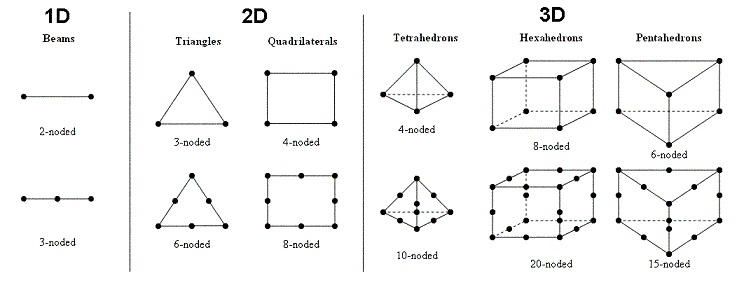
\includegraphics[width=1\linewidth]{FEMelement}
\end{figure}
\begin{center}
	\small fig 3.1 Basic finite elements.
\end{center}

The domain discretization is always considered as the preprocessing task because it can be completely seperated from the other steps. Therefore, many well-developed finite element programs are created and open sourced to us. In this project I used gmsh as the mesh generator to discretize the entire domain for 2D cases.

\subsection{Selection of Interpolation Functions}
The second step of finite element analysis is the selection of an interpolation function that provides an approxiamation of the unknown solution within an element. The interpolation can be a polynomial of first (linear), second (quadratic), third (cubic) or higher order. The higher the order is, the more accurate the interpolation can be, while the interpolation formula will be more complicated. Once the order of the polynomial is selected, we can derive an expression for the unknown solution in an element in the following form:
\begin{equation}
\widetilde{\phi} = \sum_{i=1}^{N} N^e_j {\phi}^e_j = \{N^e\}^T\{\phi^e\}
\end{equation}
where n is the number of nodes in each element;  ${{\phi}^e_j}$ is the value of ${\phi}$ at node j in the element; and ${N^e_j}$ is the interpolation function (or basis function) for node j which has the polynomial form. The most important feature of functions ${N^e_j}$ is that they are nonzero only within the element e, and outside this element they must vanish, due to the feature of Hilbert space. Another thing we need to note is that the order of the interpolation functions ${N^e_j}$ is the same as the order of element. In this paper I used Linear, quadratic and cubic interpolation for 1D problem and only linear interpolation for 2d cases.   


\section{Formulation and Boundary condition}
\subsection{Formulation via Ritz Method}
The third step in a finite element analysis is to formulate the system of equations. Reconsider the equation (1) and for simplicity assume that the problem is real valued. When the entire domain is discretized into subdomains, The \textit{functional} function F(${\widetilde{\phi}}$) defined in (3) can be expressed as
\begin{equation}
F(\widetilde{\phi}) = \sum_{e=1}^{M} F^e(\widetilde{\phi}^e) 
\end{equation}
where M is the number of elements making up the entire domian and
\begin{equation}
F^e(\widetilde{\phi}^e) = \frac{1}{2} \int_{\Omega^e} \widetilde{\phi}^e \mathcal{L} \widetilde{\phi}^e d\Omega -\int_{\Omega^e} f \widetilde{\phi}^e d\Omega
\end{equation}
where ${{\Omega^e}}$ is the domain of each element. Substituting the interpolation scheme (10) into (12), we obtain
\begin{equation}
F^e =  \{\phi^e\}^T \{\frac{1}{2} \int_{\Omega^e}\{N^e\}\mathcal{L}\{N^e\}^Td{\Omega}\{\phi^e\} - \int_{\Omega^e}f\{N^e\}d{\Omega}\}
\end{equation}
which can be written in matrix form as 
\begin{equation}
F^e = \frac{1}{2} \{\phi^e\}^T[K^e]\{\Phi^e\} - \{\Phi^e\}^T\{b^e\}
\end{equation}
where ${[K^e]}$ is an n ${\times}$ n matrix while {b$^e$} an n  ${\times}$ 1 vector, n is the number of nodes in an element. The elements in ${[K^e]}$ and {b$^e$} are
\begin{equation}
K^e_{ij} = \int_{\Omega^e}N^e_i \mathcal{L}N^e_j d\Omega
\end{equation}
\begin{equation}
b^e_i = \int_{\Omega^e}fN^e_i d\Omega
\end{equation}
Note that since ${\mathcal{L}}$ is self-adjoint, matrix [K$^e$] is symmetric. Substituting (14) to (11), we can obtain the formula of F in the entire domain as
\begin{equation}
F(\widetilde{\phi}) = \sum_{e=1}^{M} (\frac{1}{2}\{\phi^e\}^T[K^e]\{\phi^e\} - \{\phi^e\}^T\{b^e\})
\end{equation}
By performing the summation and replacing the local node numbers with the global node numbers, (17) can be written as
\begin{equation}
F = \frac{1}{2}\{\phi\}^T[K]\{\phi\}-\{\phi\}^T\{b\}
\end{equation}
where [K] is an N ${\times}$ N matrix, with N being the total number of nodes in the entire domain; ${\{\phi\}}$ is an N ${\times}$ 1 vector referring to the unknown value on these nodes;  ${\{b\}}$ is the N ${\times}$ 1 vector standing for source term.  
According to variational theorem, the solution to the system of equations can be obtained by imposing the stationarity requirement $\delta$ F = 0. Here we can equivalently set the partial derivative of F with respect to $\phi_i$ to be zero:

\begin{equation}
\frac{\partial F}{\partial \phi_i} = \sum_{j=1}^{N}K_{ij}\phi_j - b_i = 0 \hspace{0.5cm} i = 1,2,...,N
\end{equation}
or in a matrix form,
\begin{equation}
[K]\{\phi\} = \{b\}
\end{equation}
With equation (20), we are able to solve the problem via LU decomposition and backward/forward substitution.

\subsection{Application of Boundary Condition}
Before we solve the system of equations, we need to apply the required boundary conditions. There are three kinds of boundary conditions that are often encountered: Dirichlet, Neumann and Robin's boundary condition. The Dirichlet condition is an \textit{essential} boundary condition that must be imposed explicitely; in contrast, the Neumann condition is always satisfied implicitly and automatically in the solution process, hence Neumann condition is also called the \textit{natural boundary condition}. For Robin condition, since it is the linear combination of Dirichlet and Neumann condition, emplicitely implementing is also needed.

\section{Numerical Solution via Finite Element Analysis}
In the foregoing sections I introduced the steps of solving one boundary-valued problem via FEM analytically and numerically. Hence in this section, I will apply the Finite Element Analysis to one-dimensional and two-dimensional problems with both Dirichlet and Neumann boundary conditions, including electrostatic and transmission line cases.
\subsection{One-dimensional Poisson Equation}
At the first beginning I implement the Finite Element analysis to 1D poisson equation
\begin{equation}
-\frac{d^2\phi}{dt^2} = \pi^2sin(\pi x) \hspace{0.5cm} 0<x<L 
\end{equation} 
Here L = 1, x $\in$[0,L] is the entire domain, with Dirichlet boundary condition
\begin{equation}
\phi|_{x=0} = \phi|_{x=L} = 0
\end{equation}
From the boundary condition we can easily find the analytical solution is 
\begin{equation}
\phi = sin(\pi x) \hspace{0.5cm} 0<x<L 
\end{equation}
Firstly I choose linear element and interpolation, which is 
\begin{equation}
\phi^e(x) = \sum_{j=1}^{2}N_j^e(x)\phi^e_j
\end{equation}
where N$^e_j$ denotes the interpolation function given by
\begin{align*}
N^e_1(x) = \frac{x^e_2-x}{l^e} \hspace{0.5cm} and \hspace{0.5cm} N^e_2(x) = \frac{x-x^e_1}{l^e}
\end{align*}
where l$^e$ is the length of element. Then, formulating via the Ritz method. By intergrating over the element I calculate K$^e_{ij}$ and b$^e_j$ from
\begin{equation}
K^e_{ij} =\int_{x_1^e}^{x_2^e}\frac{dN^e_i}{dx} \frac{dN^e_j}{dx} dx
\end{equation}
\begin{equation}
b^e_j = \int_{x_1^e}^{x_2^e}N_i^efdx
\end{equation}
where f = $\pi^2$sin($\pi$x) here, as the source term. 
The next step is assemblying to form the system of equations by a summation over all elements and then an imposition of the stationarity requirement:
\begin{equation}
\sum_{e=1}^{M}([\overline{K}^e]\{\overline{\phi}^e\} - \{\overline{b}^e\}) = \{0\}
\end{equation}
Here I discretized the entire domain into M = 18 elements, with 19 nodes. Having obtained [K] and {b}, I applied the Dirichlet boundary condition by setting the value of $\phi$ at the boundary points to be zero, hence the size of [K] and {b} reduced by 2. Then I solved the vector {$\phi$} by LU decomposition. I also used finite difference menthod to solve the same problem with the same discretization, which is shown in figure 5.1
\begin{figure}[h]
	\centering
	\includegraphics[width=1\linewidth]{1Dlinear}
\end{figure}
\begin{center}
	\small fig 5.1 FEM and FD solution to one-dimensional Poisson's equation
\end{center} 
To exam the accuracy of FEM and FD, I calculated the L$_\infty$ norm of it. Note that FEM's solution is extremely accurate on each node, hence I choose h$_e$ = h/N as the size of interval to sample the interpolared solution on the whole region. The error distribution (compared with analytical solution with the same sampling frequency) is shown in fig 5.2
\begin{figure}[h]
	\centering
	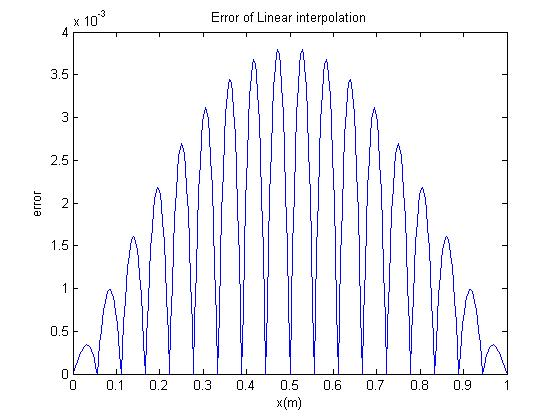
\includegraphics[width=1\linewidth]{1dLinearError}
\end{figure}
\begin{center}
	\small fig 5.2 Error distribution from linear interpolation 
\end{center} 
From figure 5.2, the L$_\infty$ norm is 0.0038, while the L$_\infty$ norm of finite difference method is 0.0025. The error of these methods shares the same order of magnitudes. Hence linear interpolation is not with a very high accuracy. To study how the order of interpolation affects the accuracy, I tried quadratic and cubic interpolation as
\begin{equation}
\phi^e_{q}(x) = \sum_{j=1}^{3}N_j^e(x)\phi^e_j \hspace{0.2cm} and \hspace{0.2cm} \phi^e_{c}(x) = \sum_{j=1}^{4}N_j^e(x)\phi^e_j
\end{equation}
where N$^e_j$ for quadratic interpolation is given by
\begin{align*}
N^e_1(x) = \frac{(x-x^e_2)(x-x^e_3)}{(x^e_1-x^e_2)(x^e_1-x^e_3)} \\
N^e_2(x) = \frac{(x-x^e_1)(x-x^e_3)}{(x^e_2-x^e_1)(x^e_2-x^e_3)} \\
N^e_3(x) = \frac{(x-x^e_1)(x-x^e_2)}{(x^e_3-x^e_1)(x^e_3-x^e_2)}
\end{align*}
while N$^e_j$ for cubic interpolation is given by
\begin{align*}
N^e_1(x) = \frac{(x-x^e_2)(x-x^e_3)(x-x^e_4)}{(x^e_1-x^e_2)(x^e_1-x^e_3)(x^e_1-x^e_4)} \\
N^e_2(x) = \frac{(x-x^e_1)(x-x^e_3)(x-x^e_4)}{(x^e_2-x^e_1)(x^e_2-x^e_3)(x^e_2-x^e_4)} \\
N^e_3(x) = \frac{(x-x^e_1)(x-x^e_2)(x-x^e_4)}{(x^e_3-x^e_1)(x^e_3-x^e_2)(x^e_3-x^e_4)} \\
N^e_4(x) = \frac{(x-x^e_1)(x-x^e_2)(x-x^e_3)}{(x^e_4-x^e_1)(x^e_4-x^e_2)(x^e_4-x^e_3)}
\end{align*}
Using the same size of discretization as N = 18, the L$\infty$ norm of these two interpolation are 3.350e-4 and 3.769e-5, respectively, which is much smaller than both FEM with linear interpolation and finite difference method. The error distribution of the two kinds of interpolation is shown in figure 5.3 and 5.4
\begin{figure}[h]
	\centering
	\includegraphics[width=1\linewidth]{1DQuadraticError}
\end{figure}
\begin{center}
	\small fig 5.3 Error distribution from quadratic interpolation
\end{center} 
\begin{figure}[h]
	\centering
	\includegraphics[width=1\linewidth]{1DCubicError}
\end{figure}
\begin{center}
	\small fig 5.4 Error distribution from cubic interpolation
\end{center} 
I then test the scheme for convergence by doing seven runs. I start with N = 18 (with 19 nodes) and find the L$_\infty$ norm of finite differece method, FEM with linear interpolation, quadratic interpolation as well as cubic interpolation. Then I halve the size of element and repeat the same procedure for 7 runs. The results is shown in Table 5.1 to 5.4

\begin{center}
	\begin{tabular}{| c | c | c | c | c | c |}
		\hline
		Num	& $\lVert err \lVert$$_{l^\infty}$ & ${l^\infty}$ ratio&  Num	& $\lVert err \lVert$$_{l^\infty}$ & ${l^\infty}$ ratio \\ \hline
		18 & 0.0025 & 4.0046 & 288 & 9.916e-6 & 4.0000\\ \hline
		36 & 6.349e-4 & 4.0011 & 576 & 2.479e-6 & 4.0000 \\ \hline
		72 & 1.587e-4 & 4.0003 & 1152 & 6.198e-7 & 4.0000 \\ \hline
		144 & 3.966e-5 & 4.0001 & 2304 & 1.549e-7 &  \\ \hline
	\end{tabular}
\end{center}
\begin{center}
	\small Table 5.1 Error of L$^\infty$ norm  of finite difference method
\end{center}

\begin{center}
	\centering
	\begin{tabular}{| c | c| c | c | c | c |}
		\hline
		Num	& $\lVert err \lVert$$_{l^\infty}$ & ${l^\infty}$ ratio&  Num	& $\lVert err \lVert$$_{l^\infty}$ & ${l^\infty}$ ratio \\ \hline
		18 & 0.0038 & 3.9867 & 288 & 1.487e-5 & 4.0000\\ \hline
		36 & 9.508e-4 & 3.9967 & 576 & 3.719e-6 & 4.0000 \\ \hline
		72 & 2.379e-4 & 3.9992 & 1152 & 9.296e-7 & 4.0000 \\ \hline
		144 & 5.949e-5 & 3.9998 & 2304 & 2.324e-7 &  \\ \hline
	\end{tabular}
\end{center}
\begin{center}
	\small Table 5.2 Error of L$^\infty$ norm of FEM with linear interpolation
\end{center}

\begin{center}
	\begin{tabular}{| c | c | c | c | c | c |}
		\hline
		Num	& $\lVert err \lVert$$_{l^\infty}$ & ${l^\infty}$ ratio&  Num	& $\lVert err \lVert$$_{l^\infty}$ & ${l^\infty}$ ratio \\ \hline
		 18 & 3.350e-4 & 7.8897 & 288 & 8.326e-8 &7.9996\\ \hline
	     36 & 4.246e-5 & 7.9768 & 576 & 1.041e-8 & 8.0000 \\ \hline
		 72 & 5.323e-6 & 7.9930 & 1152 & 1.301e-9 &  \\ \hline
		 144 & 6.660e-7 & 7.9985 &   &  &  \\ \hline
	\end{tabular}
\end{center}
\begin{center}
	\small Table 5.3 Error of L$^\infty$ norm of FEM with quadratic interpolation
\end{center}


\begin{center}
	\begin{tabular}{| c | c | c | c  |}
		\hline
		Number of element	& $\lVert err \lVert$$_{l^\infty}$ & ${l^\infty}$ ratio \\ \hline
		18 & 3.768e-5 & 15.5501 \\ \hline
		36 & 2.424e-6 & 15.8874  \\ \hline
		72 & 1.526e-7 & 15.9695 \\ \hline
		144 & 9.553e-9 &  \\ \hline
	\end{tabular}
\end{center}
\begin{center}
	\small Table 5.4 Error of L$^\infty$ norm of FEM with cubic interpolation
\end{center}

From the convergence analysis we can see that both finite difference method and FEM with linear interpolation are of 2$^{nd}$ order accuracy, quadratic is of 3$^{rd}$ order accuracy while cubic is of 4$^{th}$ order accuracy. Note that for quadratic and cubic interpolation I didn't try as much as 7 runs, that's because the error decreases really fast when I halve the size of element, when it reaches to the order of round-off error as 1e-10, the result will be contaminated. 

\subsection{Two-dimensional Poisson Equation}
With all the effort on one-dimensional case, now we can move to two-dimensional problems. For electromagnetic problems, we always solve it in frequence domain by assuming the EM wave is time-harmonic. In general case, the 2D anisotropic Helmholtz equation can be written as
\begin{equation}
-\frac{\partial}{\partial x} \bigg(\alpha_x \frac{\partial\phi}{\partial x}\bigg) -\frac{\partial}{\partial y} \bigg(\alpha_y \frac{\partial\phi}{\partial y}\bigg) + \beta \phi= f
\end{equation}
Where $\phi$ can be electric field, magnetic field, potential or vector potential which satisfies Lorentz condition. 
At the first beginning I solve the equation with the simplest case given as following:
\begin{equation}
-\frac{\partial^2 \phi}{\partial x^2}-\frac{\partial^2 \phi}{\partial y^2} = 2\pi^2 sin(\pi x)cos(\pi y)
\end{equation}
where x, y defined on [0,1]$\times$[0,1], with the boundary condition
\begin{align*}
\phi|_{x = 0} = \phi|_{x = 1} = 0 \hspace{0.2cm} and \hspace{0.2cm} \frac{\partial \phi}{\partial n}|_{y = 0} = \frac{\partial \phi}{\partial n}|_{y = 1} = 0
\end{align*}
Therefore the analytical solution is $\phi$ = sin($\pi$x)cos($\pi$y). Solved with linear interpolation, result is shown in figure 5.5, while the analytical solution is shown in figure 5.6
\begin{figure}[h]	
	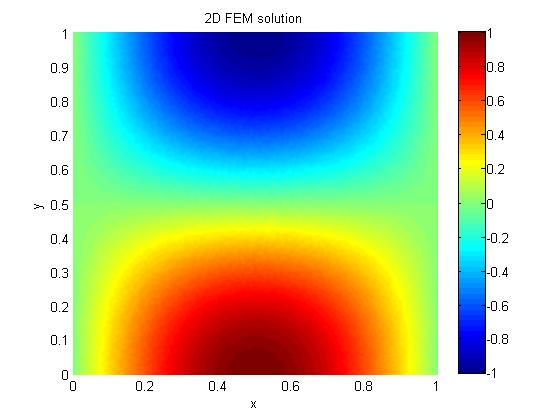
\includegraphics[width=1\linewidth]{2DPoissonFEM}
\end{figure}
\begin{center}
	\small fig 5.5 FEM solution to 2D Poisson equation 
\end{center} 
\begin{figure}[h]
	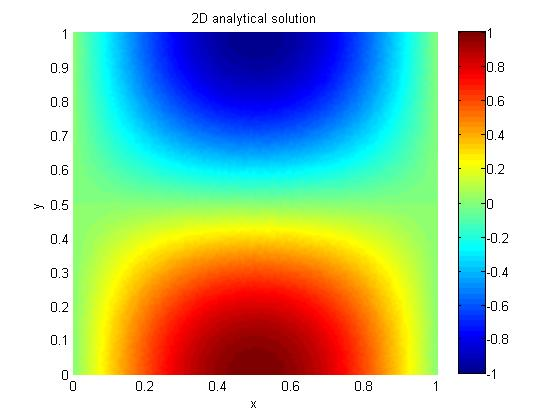
\includegraphics[width=1\linewidth]{2DPoissonAnalytical}
\end{figure}
\begin{center}
	\small fig 5.6 Analytical solution to 2D Poisson equation
\end{center} 

\subsection{Electrostatic Problem:  Electric Potential distribution on a Microstrip Line}
Microstrip Line is widely used in communication system. It consists of a substrate made of dielectric material (such as FR-4) with a metal strip on the top surface of it. The size of it is always in micro-meter, hence is called "microstrip line". It can be a type of electrical transmission line implemented on printed board circuit technology or multi-chip modules (MCM). Transmission line acts as an interconnect between various devices on platform. When we excite one terminal of it, the wave will propagate through it to other terminals. Figure 5.7 shows the transection of the basic model of a microstrip line with E and H field distribution.

In this section, I will solve the electric potential distribution on a microstrip line.
\begin{figure}[h]
	\centering
	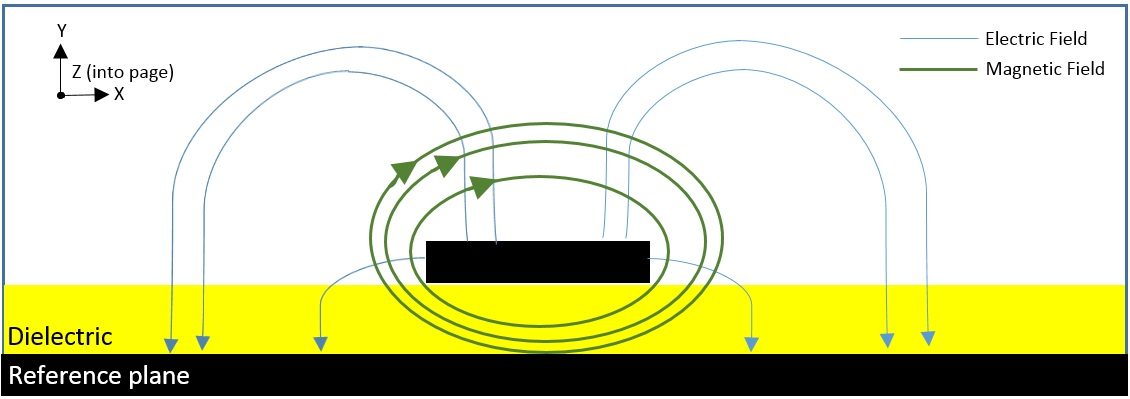
\includegraphics[width=0.8\linewidth]{Microstrip_fieldlines}
\end{figure}
\begin{center}
	\small fig 5.7 E and H field distribution on a microstrip line 
\end{center} 
The two-dimensional electrostatic field problems are governed by the two-dimensional Poisson equation
\begin{equation}
-\frac{\partial}{\partial x}(\epsilon_r\frac{\partial \phi}{\partial x})-\frac{\partial}{\partial y}(\epsilon_r\frac{\partial \phi}{\partial y}) = \frac{\varrho}{\epsilon_0}
\end{equation}
where $\varrho$ denotes the charge density, and $\epsilon_r$ denotes the relative permittivity. The geometry and mesh of the microstrip model is shown in fig 5.8 and fig 5.9
\begin{figure}[h]
	\centering
	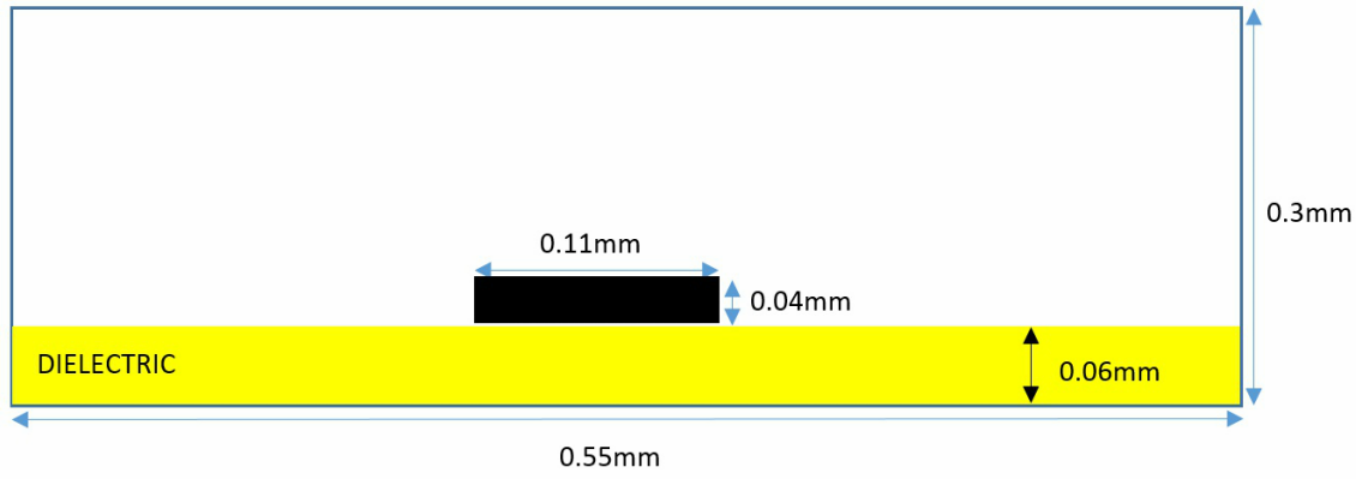
\includegraphics[width=0.8\linewidth]{Microstrip_geometry}
\end{figure}
\begin{center}
	\small fig 5.8 Geometry information of the microstrip line 
\end{center} 
\begin{figure}[h]
	\centering
	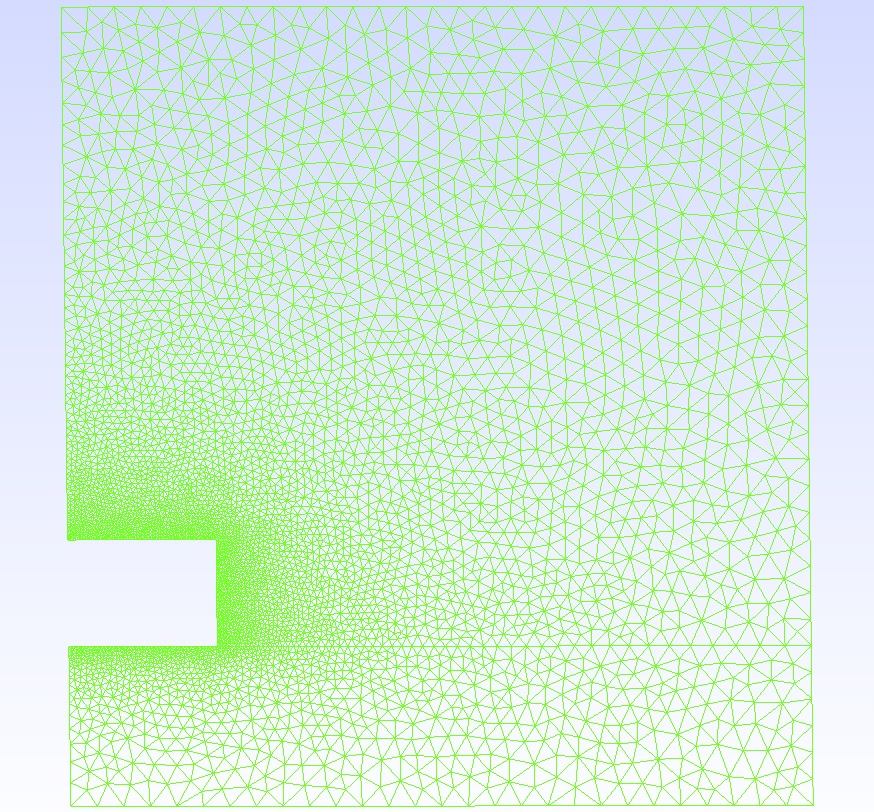
\includegraphics[width=0.8\linewidth]{MicrostripeMesh}
\end{figure}
\begin{center}
	\small fig 5.9 mesh of the microstrip line
\end{center} 
Note that since the model, and  governing equations are symmetric, hence I can reduce the solution domain by half by applying the homogeneous Neumann boundary condition at the plane of symmetry.

From figure 5.8, the width of the metal is 0.11mm, with thickness be 0.04mm. I used copper as the metal whose conductivity if 4.0$\times$10$^7$ S/m. The height of substrate is 0.06mm with the material whose relative permittivity is 3.\\

As a simplification we can assume that both electric and magnetic fields are orthogonal to z-direction, in which the wave propagates in transverse electro-magnetic mode (TEM). Therefore we can decompose the transmission line into discrete segments along the z-direction and analyze the distribution on the cross section. \\

The boundary condition of this model requires classified discussion. First is the boundary on the surface of metal. For a electrostatic problem, since I am interested in electric potential distribution, I can set the potential on the surface to be 1 V because it is equipotential on the surface of good conductors, and the potential to be 0 on the ground surface. On the interface of substrate and air, as potentil jump can lead to infinite electric field intensity, it must follow the Neumann boundary as $\frac{\partial \phi}{\partial n} = 0$. The most difficult one is the outer boundary. For most of the cases microstrip line is within an relatively open or unbounded domain, which means field must vanish at boundaries and no reflection is allowed. Hence, a perfect matching layer will be the optimal choice, which is often used in radiation and antenna problems. For simplicity here I let the outer box to be large enough and use Dirichlet boundary contion. The result of electric potential distribution is shown in figure 5.10.
\begin{figure}[h]
	\centering
	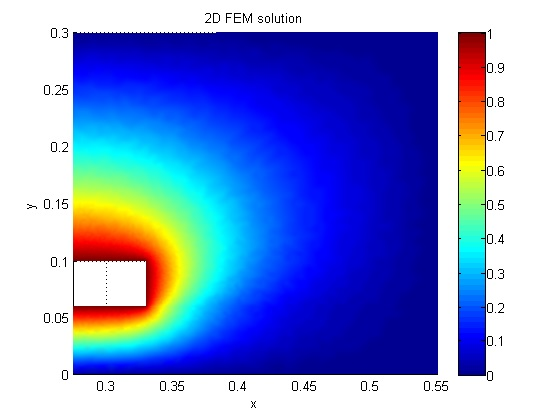
\includegraphics[width=1\linewidth]{Microstrip_solved}
\end{figure}
\begin{center}
	\small fig 5.10 FEM solution of electric potention distribution on a microstrip line 
\end{center} 

This time I have no way to obtain the analytical solution. For checking the correctness of FEM solution I solve the same problem via COMSOL. The result from COMSOL is shown in figure 5.11. We can have a intuitive impression that the result from my solver is fairly close to the result solved by COMSOL. Note that we don't care about the potential distribution inside the metal while COMSOL still calculate them out.

\begin{figure}[h]
	\centering
	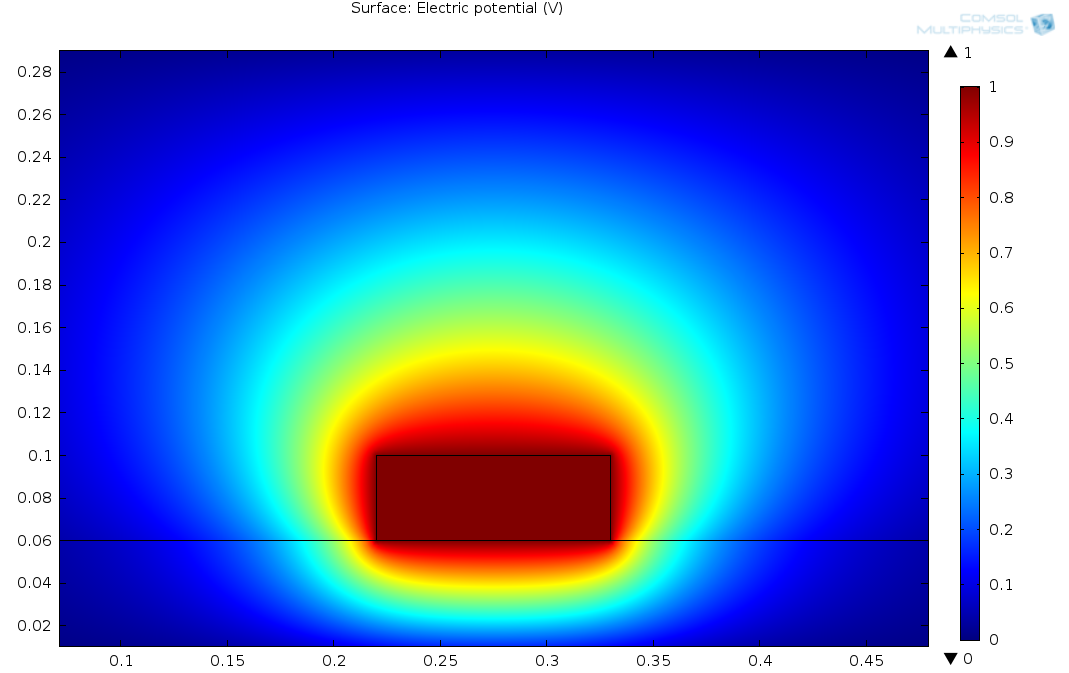
\includegraphics[width=1\linewidth]{MicrostripComsol}
\end{figure}
\begin{center}
	\small fig 5.11 electric potention distribution on a microstrip line from COMSOL.
\end{center} 

\subsection{FEM to Quasistatic Problem: Analysis of Multiconductor Transmission Lines}
Analysis of multiconductor transmission lines is an important problem for the design of high-frequency integrated circuits. For transmission lines made of lossy conductions, we can employ a quasistatic analysis that keeps the conduction current and ignores the displacement current introduced by electromagnetic induction. With this approximation, ${\textbf{E}}$ $\approx$ -j$\omega$${\textbf{A}}$, where $\textbf{E}$ is the electric field,  $\omega$ is the angular frequency and $\textbf{A}$ is the vector potential defined by ${\textbf{B}}$ = $\bigtriangledown$$\times$${\textbf{A}}$. From Maxwell's equations, we can obtain
\begin{equation}
\bigtriangledown \times(\frac{1}{\mu_r}\bigtriangledown \times A_z \hat{z})+j \omega \mu_0 \sigma A_z \hat{z} = \mu_0 \bar{J}_{imp} \hat{z}
\end{equation}
where $\sigma$ denotes the conductivity of the lossy conductors and $\hat{J}$$_{imp}$ is the impressed current along the longitudinal direction (for this problem is z direction). Conductors are made of aluminum-oxide with $\sigma$ = 3.6$\times$10$^7$ and $\mu_r$ = 1. With relation  ${\textbf{E}}$ $\approx$ -j$\omega$${\textbf{A}}$, (32) can be written as
\begin{equation}
-\frac{\partial^2 {A_z}}{\partial {x^2}} - \frac{\partial^2 {A_z}}{\partial {y^2}} + j \omega \mu _0 \sigma A_z = \mu_0 \sigma E_{imp}
\end{equation}
The information of geometry and mesh of the multicondutors transmission line model are shown in figure 5.12 and 5.13
\begin{figure}[h]
	\centering
	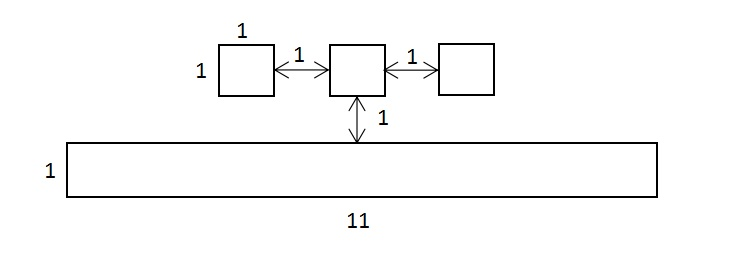
\includegraphics[width=1\linewidth]{TLmodel}
\end{figure}
\begin{center}
	\small fig 5.12 Geometry information of the multiconductor transmission line model
\end{center} 
\begin{figure}[h]
	\centering
	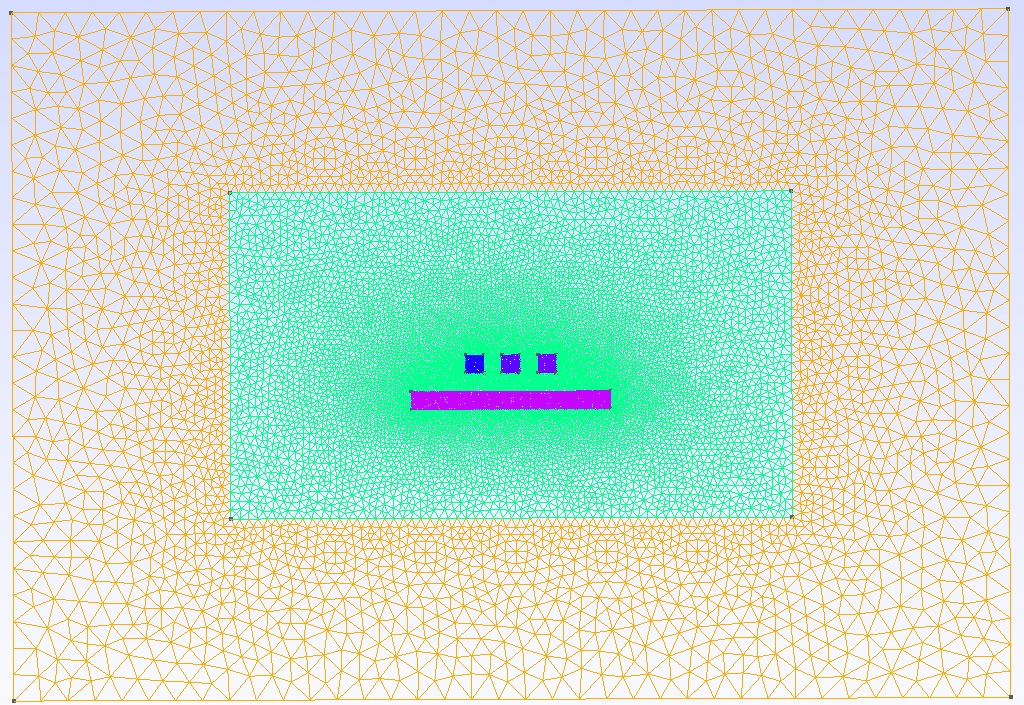
\includegraphics[width=0.8\linewidth]{TLMesh}
\end{figure}
\begin{center}
	\small fig 5.13 Mesh information of the multiconductor transmission line model
\end{center} 
Note that I used two region of mesh, the outer one is of coarse mesh size while the inner one is of finer mesh size. The boundary condition here for any interface can be set as Neumann boundary condition. With the system of elements, I excited the conductors one by one with E$_{imp}$ = 1 and $\omega$ = 10 MHz to  obtain the electric field distribution among the region. As usual, I compare my numerical solution with the result from COMSOL, as is shown in figure 5.14 to 5.17 (Here I only show the result when excit)

\begin{figure}[h]
	\centering
	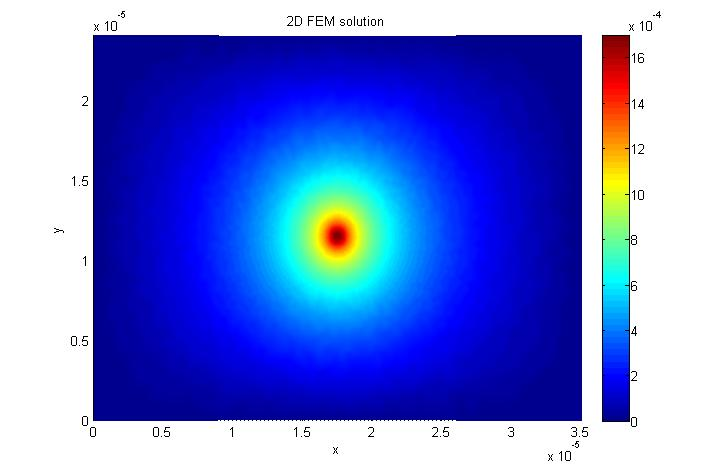
\includegraphics[width=0.8\linewidth]{10MHz2}
\end{figure}
\begin{center}
	\small fig 5.14 E field distribution from my solution when excite conductor 2
\end{center} 
\begin{figure}[h]
	\centering
	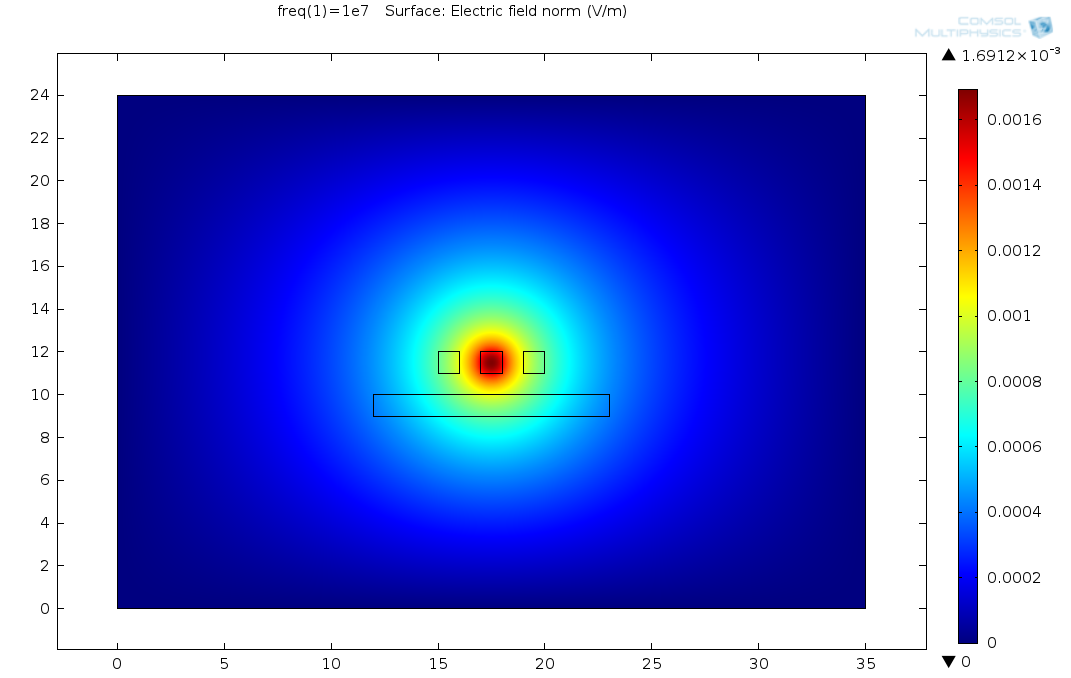
\includegraphics[width=0.8\linewidth]{10MHzCOMSOL2}
\end{figure}
\begin{center}
	\small fig 5.15 E field distribution from COMSOL when excite conductor 2
\end{center} 

\begin{figure}[h]
	\centering
	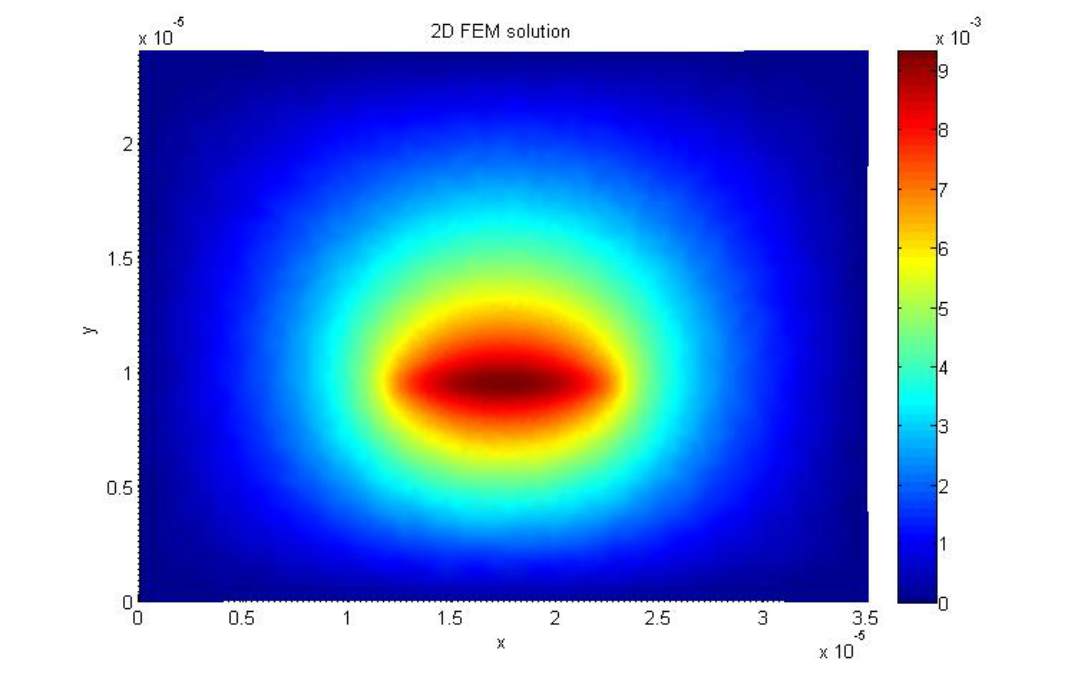
\includegraphics[width=0.8\linewidth]{10MHz4}
\end{figure}
\begin{center}
	\small fig 5.16 E field distribution from my solution when excite conductor 4
\end{center} 
\begin{figure}[h]
	\centering
	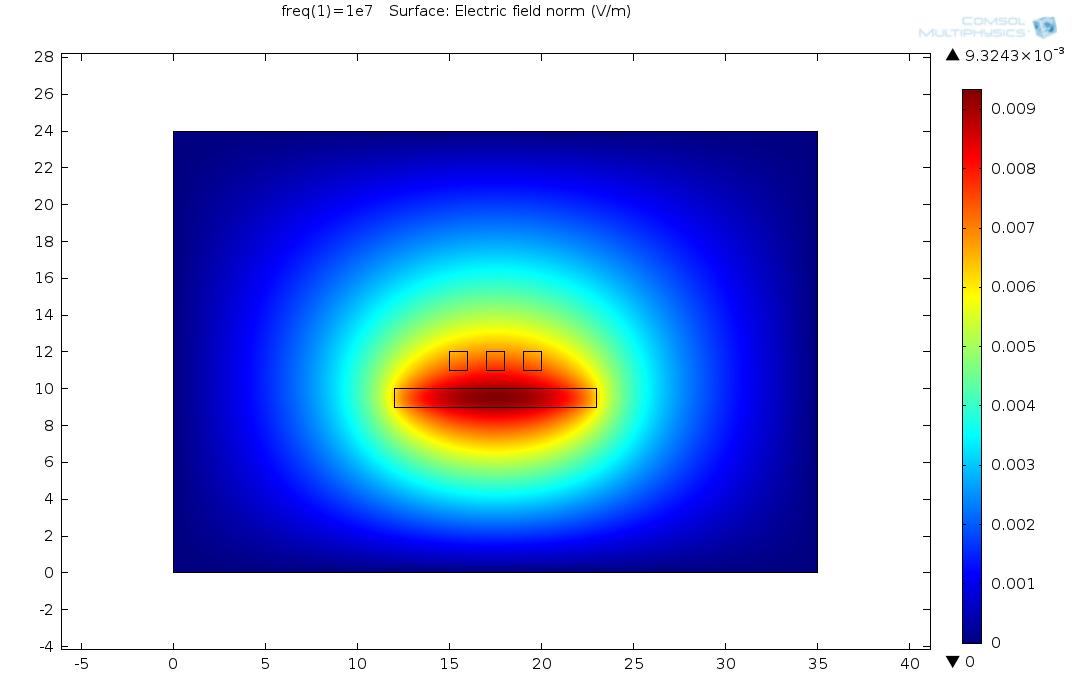
\includegraphics[width=0.9\linewidth]{10MHzCOMSOL4}
\end{figure}
\begin{center}
	\small fig 5.17 E field distribution from COMSOL when excite conductor 4
\end{center} 
Compare the solutions from my FEM solver and COMSOL, they are fairly close to each other. Hence My algorithm is relatively reliable like commercial softwares.
% An example of a floating figure using the graphicx package.
% Note that \label must occur AFTER (or within) \caption.
% For figures, \caption should occur after the \includegraphics.
% Note that IEEEtran v1.7 and later has special internal code that
% is designed to preserve the operation of \label within \caption
% even when the captionsoff option is in effect. However, because
% of issues like this, it may be the safest practice to put all your
% \label just after \caption rather than within \caption{}.
%
% Reminder: the "draftcls" or "draftclsnofoot", not "draft", class
% option should be used if it is desired that the figures are to be
% displayed while in draft mode.
%
%\begin{figure}[!t]
%\centering
%\includegraphics[width=2.5in]{myfigure}
% where an .eps filename suffix will be assumed under latex, 
% and a .pdf suffix will be assumed for pdflatex; or what has been declared
% via \DeclareGraphicsExtensions.
%\caption{Simulation results for the network.}
%\label{fig_sim}
%\end{figure}

% Note that the IEEE typically puts floats only at the top, even when this
% results in a large percentage of a column being occupied by floats.


% An example of a double column floating figure using two subfigures.
% (The subfig.sty package must be loaded for this to work.)
% The subfigure \label commands are set within each subfloat command,
% and the \label for the overall figure must come after \caption.
% \hfil is used as a separator to get equal spacing.
% Watch out that the combined width of all the subfigures on a 
% line do not exceed the text width or a line break will occur.
%
%\begin{figure*}[!t]
%\centering
%\subfloat[Case I]{\includegraphics[width=2.5in]{box}%
%\label{fig_first_case}}
%\hfil
%\subfloat[Case II]{\includegraphics[width=2.5in]{box}%
%\label{fig_second_case}}
%\caption{Simulation results for the network.}
%\label{fig_sim}
%\end{figure*}
%
% Note that often IEEE papers with subfigures do not employ subfigure
% captions (using the optional argument to \subfloat[]), but instead will
% reference/describe all of them (a), (b), etc., within the main caption.
% Be aware that for subfig.sty to generate the (a), (b), etc., subfigure
% labels, the optional argument to \subfloat must be present. If a
% subcaption is not desired, just leave its contents blank,
% e.g., \subfloat[].


% An example of a floating table. Note that, for IEEE style tables, the
% \caption command should come BEFORE the table and, given that table
% captions serve much like titles, are usually capitalized except for words
% such as a, an, and, as, at, but, by, for, in, nor, of, on, or, the, to
% and up, which are usually not capitalized unless they are the first or
% last word of the caption. Table text will default to \footnotesize as
% the IEEE normally uses this smaller font for tables.
% The \label must come after \caption as always.
%
%\begin{table}[!t]
%% increase table row spacing, adjust to taste
%\renewcommand{\arraystretch}{1.3}
% if using array.sty, it might be a good idea to tweak the value of
% \extrarowheight as needed to properly center the text within the cells
%\caption{An Example of a Table}
%\label{table_example}
%\centering
%% Some packages, such as MDW tools, offer better commands for making tables
%% than the plain LaTeX2e tabular which is used here.
%\begin{tabular}{|c||c|}
%\hline
%One & Two\\
%\hline
%Three & Four\\
%\hline
%\end{tabular}
%\end{table}


% Note that the IEEE does not put floats in the very first column
% - or typically anywhere on the first page for that matter. Also,
% in-text middle ("here") positioning is typically not used, but it
% is allowed and encouraged for Computer Society conferences (but
% not Computer Society journals). Most IEEE journals/conferences use
% top floats exclusively. 
% Note that, LaTeX2e, unlike IEEE journals/conferences, places
% footnotes above bottom floats. This can be corrected via the
% \fnbelowfloat command of the stfloats package.




\section{Conclusion}
Through this paper, I implemented finite element method for solving the following problems: 
\begin{itemize}
	\item 1-dimensional Poisson equation: I solved it with FEM and finite difference method. The convergence analysis shows that with linear interpolation and center-difference, both FEM and FD have a 2$^{nd}$ order accuracy; with quadratic interpolation FEM has a 3$^{rd}$ order accuracy; while with cubic interpolation FEM has a 4$^{th}$ order accuracy.
	\item 2-dimensional Poisson equation: I solved it with FEM and compared with analytical solution. 
	\item 2-dimensional Microstrip Line: I solved it with FEM and compared with result from COMSOL.
	\item 2-dimensional Transmission Line: I solved it with FEM and compared with result from COMSOL.
\end{itemize}
The comparison shows my FEM algorithm is reliable for the correct solution which is close to the commercial software. However, it also took much longer time than COMSOL when solving the two-dimensional cases. Hence more modification is needed for improving the performance.

% if have a single appendix:
%\appendix[Proof of the Zonklar Equations]
% or
%\appendix  % for no appendix heading
% do not use \section anymore after \appendix, only \section*
% is possibly needed

% use appendices with more than one appendix
% then use \section to start each appendix
% you must declare a \section before using any
% \subsection or using \label (\appendices by itself
% starts a section numbered zero.)
%


% use section* for acknowledgment
\section*{Acknowledgment}

This paper would not have been possible without the zealous support from Prof. Mary Pugh as well as my supervisor, Prof. Piero Triverio. Prof. Pugh helps me with convegence analysis of higher order element and Prof. Triverio helps me with understanding physics model of multiconductor Transmission Line. 


% Can use something like this to put references on a page
% by themselves when using endfloat and the captionsoff option.
\ifCLASSOPTIONcaptionsoff
  \newpage
\fi



% trigger a \newpage just before the given reference
% number - used to balance the columns on the last page
% adjust value as needed - may need to be readjusted if
% the document is modified later
%\IEEEtriggeratref{8}
% The "triggered" command can be changed if desired:
%\IEEEtriggercmd{\enlargethispage{-5in}}

% references section

% can use a bibliography generated by BibTeX as a .bbl file
% BibTeX documentation can be easily obtained at:
% http://mirror.ctan.org/biblio/bibtex/contrib/doc/
% The IEEEtran BibTeX style support page is at:
% http://www.michaelshell.org/tex/ieeetran/bibtex/
%\bibliographystyle{IEEEtran}
% argument is your BibTeX string definitions and bibliography database(s)
%\bibliography{IEEEabrv,../bib/paper}
%
% <OR> manually copy in the resultant .bbl file
% set second argument of \begin to the number of references
% (used to reserve space for the reference number labels box)
\begin{thebibliography}{1}
	
	\bibitem{FEM}
	J.M.Jin, \emph{The Finite Element Method in Electromagnetics}, 3rd~ed. \hskip 3em plus
	0.5em minus 0.4em\relax New York : John Wiley and Sons, 2015.
	
	%\bibitem{FEM2}
	%J.M.Jin, \emph{The Finite Element Method in Electromagnetics}, 2nd~ed. \hskip 3em plus
	%0.5em minus 0.4em\relax New York : John Wiley and Sons, 2002.
	
\end{thebibliography}
% biography section
% 
% If you have an EPS/PDF photo (graphicx package needed) extra braces are
% needed around the contents of the optional argument to biography to prevent
% the LaTeX parser from getting confused when it sees the complicated
% \includegraphics command within an optional argument. (You could create
% your own custom macro containing the \includegraphics command to make things
% simpler here.)
%\begin{IEEEbiography}[{\includegraphics[width=1in,height=1.25in,clip,keepaspectratio]{mshell}}]{Michael Shell}
% or if you just want to reserve a space for a photo:

% if you will not have a photo at all:
\begin{IEEEbiographynophoto}{Zihan Chan}
 is currently pursuing the M.A.Sc. degree in Electrical and Computer Engineering 
at University of Toronto. His research interests are in numerical methods of EM and Fluid Dynamic problems.
\end{IEEEbiographynophoto}

% insert where needed to balance the two columns on the last page with
% biographies
%\newpage

% You can push biographies down or up by placing
% a \vfill before or after them. The appropriate
% use of \vfill depends on what kind of text is
% on the last page and whether or not the columns
% are being equalized.

%\vfill

% Can be used to pull up biographies so that the bottom of the last one
% is flush with the other column.
%\enlargethispage{-5in}



% that's all folks
\end{document}


